% ---------------------------------------------------------------------------
% Springer LNCS build.  Compile with:
%     tectonic -X compile main.tex --outdir .
% The body is shared verbatim with ../ieee/main.tex; only this wrapper differs.
% ---------------------------------------------------------------------------
\documentclass[runningheads]{llncs}

\usepackage{graphicx}
\usepackage{booktabs}
\usepackage{amsmath}
\usepackage{amssymb}
\usepackage{siunitx}
\usepackage{microtype}
\usepackage[hidelinks]{hyperref}

\graphicspath{{../shared/generated/}{../shared/diagrams/}}

% siunitx v3 dropped \degree; every use in the body is in math mode.
\providecommand{\degree}{^{\circ}}

% LNCS is single-column, so a "wide" float is just a normal float.
\newenvironment{wfigure}{\figure}{\endfigure}
\newenvironment{wtable}{\table}{\endtable}
\newcommand{\tabscale}{\footnotesize}

% llncs sets a run-in \paragraph with no trailing punctuation of its own, so
% the period belongs here. IEEEtran appends its own colon and must not get one.
\newcommand{\para}[1]{\paragraph{#1.}}

% llncs uses \cite, not natbib's \citep. Map it so the shared body compiles
% unchanged under both classes.
\providecommand{\citep}[1]{\cite{#1}}

% Every experimental number in the prose is a macro; see the header comment
% in shared/generated/macros.tex for its provenance (source file, line
% numbers, and evidence grade per group).
% ---------------------------------------------------------------------------
% Numeric macros used by shared/body.tex. Every number below was read
% directly from backend/services/upwelling.py (module docstring and source,
% verified in full, all 932 lines), backend/services/sst_anomaly.py (module
% docstring, verified in full, all 209 lines), backend/services/wind_history.py
% (verified in full, 210 lines), DONE.md's "A rolling wind history" entry, and
% by running backend/tests/test_upwelling.py + backend/tests/test_wind_history.py
% directly (`uv run pytest tests/test_upwelling.py tests/test_wind_history.py -q`,
% 39 passed, no failures) -- on \AsOf{}. None of this was copied from
% research/research.md's \S1.11, which is where this paper's claim originates
% but which this project's own house rule (after repeated research.md errors
% found this session) treats as a pointer, not a source. Concretely:
%   - research.md's \S1.11 "Missing" section calls for a rolling wind history
%     experiment as not yet done. It has since been built and measured
%     (services/wind_history.py, upwelling.detect_from_history,
%     scripts/backfill_wind_history.py, scripts/measure_wind_history_
%     corroboration.py, all dated 2026-08-28 in DONE.md and in
%     sst_anomaly.py's own docstring) -- this file's "Group D" below.
%   - The same 2026-08-28 measurement is independently analysed by a
%     contemporaneous companion draft in this research program
%     (research/papers/cross_product_baseline/, not yet given ieee/springer
%     wrappers or a title) as its own "Control C", for a different purpose
%     (ruling out instantaneous wind sampling as the explanation for a
%     cross-SST-product mismatch, rather than testing whether wind averaging
%     rescues this paper's control-arm finding). Both papers report the same
%     four raw numbers from one run; see shared/body.tex's Discussion for the
%     explicit disclosure.
%
% Evidence grade for every group is noted below:
%   [ARTIFACT]        a source-code constant or a currently-passing test,
%                       reproducible on demand and not subject to drift.
%   [DATED, <date>]    a single, live run recorded with its date in a module
%                       docstring or DONE.md, naming its own reproduction
%                       script, with no stored output file committed anywhere
%                       in the repository. Cited as of that date, not as a
%                       standing fact about the current state of any field.
%   [ARTIFACT + DATED] the mechanism/infrastructure is a passing test or
%                       shipping code (Artifact); the headline number itself
%                       is a Dated measurement of a moving field. Same hybrid
%                       category research/papers/silent_failures/ uses.
% ---------------------------------------------------------------------------

\newcommand{\AsOf}{2026-09-10}

% --- Group A: fixed thresholds and constants, all [ARTIFACT, code] ---------
% backend/services/upwelling.py: COOL_ANOMALY_C (line 169), EQUATORIAL_BAND_DEG
% (line 145), COASTAL_BAND_CELLS (line 151, "two cells at ~0.25 degrees is
% ~55 km" per the code's own comment), MIN_COASTLINE_CONFIDENCE (line 162),
% NORMAL_SMOOTHING_CELLS (line 157), MAX_SST_LAG_DAYS (line 175).
\newcommand{\CoolAnomalyThreshold}{0.5}
\newcommand{\EquatorialBandDeg}{5}
\newcommand{\CoastalBandCells}{2}
\newcommand{\CoastalBandKm}{55}
\newcommand{\MinCoastlineConfidence}{0.05}
\newcommand{\NormalSmoothingCells}{3}
\newcommand{\MaxSstLagDays}{30}
% backend/services/climatology/build.py: DEFAULT_BASELINE_START/END (lines
% 59-60), DEFAULT_WINDOW_DAYS (line 67), PERCENTILES (line 72) -- confirmed
% directly against the source, not assumed from a sibling paper's macro.
\newcommand{\ClimPercentile}{10}
\newcommand{\ClimWindowDays}{5}
\newcommand{\OisstBaselineStart}{1991}
\newcommand{\OisstBaselineEnd}{2020}

% --- Group A2: the bulk wind-stress / Ekman-transport constants, all
% [ARTIFACT, code] backend/services/upwelling.py lines 135-141. ---
\newcommand{\AirDensity}{1.225}
\newcommand{\DragCoefficient}{1.3\times10^{-3}}
\newcommand{\SeawaterDensity}{1025}
\newcommand{\EarthOmega}{7.2921\times10^{-5}}

% --- Group B: the headline corroboration measurement [DATED, 2026-08-17] --
% backend/services/upwelling.py's own module docstring ("How strong the
% agreement actually is, measured") and the identical numbers repeated in its
% corroboration() method's own comment (lines 340-346). Percentages, not
% fractions, matching the docstring's own units.
\newcommand{\UpwellFavourWeak}{19.9}
\newcommand{\UpwellControlWeak}{17.2}
\newcommand{\UpwellGapWeak}{2.7}
\newcommand{\UpwellFavourStrong}{4.1}
\newcommand{\UpwellControlStrong}{3.9}
\newcommand{\UpwellGapStrong}{0.2}
\newcommand{\UpwellAnomFavour}{0.91}
\newcommand{\UpwellAnomControl}{0.60}
% Only the weak tier's control fraction is a field the live API actually
% returns (control_cool_fraction, computed lines 347-349 and returned lines
% 377-379, confirmed [ARTIFACT] by reading the code directly -- this is the
% structural fact research.md's \S1.11 calls out, independent of its dated
% value above). The strong-tier control and the mean-anomaly control are
% [DATED] numbers from the module docstring with no corresponding shipped
% field; scripts/measure_sst_corroboration.py computes them ad hoc.

% --- Group C: cross-date stability of the *same, untouched* matched
% configuration (OISST scored against its own OISST-fitted climatology,
% instantaneous wind) [DATED, three separate dates] -- used in
% \S\ref{sec:results} as the noise floor the wind-history follow-up (Group D)
% is read against. All three are "cool contrast"/"below-p10 contrast" =
% favourable-fraction minus control-fraction, in fraction units (not percent),
% exactly as scripts/measure_sst_corroboration.py and
% scripts/measure_wind_history_corroboration.py's own _contrasts() compute
% them -- NOT the same units as Group B's percentages, and not derived from
% Group B's numbers (see \S\ref{sec:methods} for why the two must not be
% subtracted from each other). Sources: backend/services/sst_anomaly.py's own
% docstring, first table (2026-08-17 row) and third table (2026-08-25, OISST
% row); the 2026-08-28 instantaneous row is shared with Group D below.
\newcommand{\MatchedWeakAugSeventeen}{0.026}
\newcommand{\MatchedWeakAugTwentyFive}{0.027}
\newcommand{\MatchedStrongAugSeventeen}{0.002}
\newcommand{\MatchedStrongAugTwentyFive}{-0.001}
% Spreads computed directly from the three matched-configuration values in
% this group and Group D (max minus min): weak = 0.027 - 0.0234 = 0.0036;
% strong = 0.002 - (-0.0061) = 0.0081.
\newcommand{\WeakCrossDateSpread}{0.0036}
\newcommand{\StrongCrossDateSpread}{0.0081}

% --- Group D: the wind-history follow-up [ARTIFACT + DATED] ---------------
% Infrastructure is [ARTIFACT]: backend/services/wind_history.py,
% upwelling.detect_from_history/_assemble_field, scripts/backfill_wind_history.py
% and scripts/measure_wind_history_corroboration.py all confirmed present and
% read in full; backend/tests/test_wind_history.py (7 tests) and
% backend/tests/test_upwelling.py's TestDetectFromHistory class (2 tests) all
% pass (`uv run pytest tests/test_upwelling.py tests/test_wind_history.py -q`,
% 39 passed, re-run on \AsOf{}).
\newcommand{\NUpwellingTests}{32}
\newcommand{\NWindHistoryTests}{7}
\newcommand{\NTotalUpwellingTests}{39}
% wind_history.py: MIN_COVERAGE_FRACTION (line 83, as a percentage),
% RETAIN_DAYS (line 71). DONE.md's "A rolling wind history" entry: the
% backfill's real span (30 backfilled timesteps, 1.21 real days -- rounded to
% "1.2" in sst_anomaly.py's own docstring, an inconsistency left visible per
% this project's own convention rather than silently resolved) against the
% originally targeted 3-day window; the _MAX_LOOKBACK_STEPS offset (30 hours)
% needed to route the backfill around copernicus_wind.py's documented
% "24 straight empty hourly placeholders" gap.
\newcommand{\WindHistoryTimesteps}{30}
\newcommand{\WindHistoryActualWindowDays}{1.2}
\newcommand{\WindHistoryTargetWindowDays}{3}
\newcommand{\WindHistoryMinCoveragePct}{50}
\newcommand{\WindHistoryLookbackHours}{30}
% The headline numbers are [DATED, 2026-08-28]: sst_anomaly.py's docstring's
% fourth section and DONE.md's own table, both read directly; reproduced by
% scripts/measure_wind_history_corroboration.py --backfill-hours 72. No
% stored output file is committed for this measurement.
\newcommand{\WindHistoryWeakInstant}{0.0234}
\newcommand{\WindHistoryWeakTrailing}{0.0182}
\newcommand{\WindHistoryStrongInstant}{-0.0061}
\newcommand{\WindHistoryStrongTrailing}{-0.0049}
% Movements computed directly from the two lines above, not new measurements:
% weak = |0.0234 - 0.0182|; strong = |-0.0061 - (-0.0049)|.
\newcommand{\WindHistoryWeakMovement}{0.0052}
\newcommand{\WindHistoryStrongMovement}{0.0012}

% ---------------------------------------------------------------------------
% Note on evidence-grading language, checked while building this table
% (\AsOf{}): silent_failures's own I.11 paragraph calls the 4.1\%/3.9\% pair
% "statistically indistinguishable". No test statistic exists anywhere in this
% codebase for that pair, or for any contrast in Group C or Group D -- there
% is no committed significance test on any of these numbers. This paper does
% not repeat that phrase; it reports the raw gaps (\UpwellGapStrong{} points)
% and the cross-date spread (Group C) instead of asserting a statistical
% conclusion the underlying measurements cannot support.
% ---------------------------------------------------------------------------


\begin{document}

\title{A Detector's Corroboration Needs a Control Arm: A Case Study in
Coastal Upwelling}

\titlerunning{A Detector's Corroboration Needs a Control Arm}

% No \orcidID: LNCS supports one, but a placeholder identifier would be a
% fabricated credential. Add the real one before submission.
\author{Deepak Krishna}
\authorrunning{D. Krishna}
\institute{MarisAI, India \\ \email{deepakkrishna2206@gmail.com}}

\maketitle

\begin{abstract}
A detector that corroborates one signal against a second, independent
observation is usually reported by its agreement rate alone, which is easy
to mistake for evidence of causation. We report a case inside a real,
shipping coastal-upwelling detector where adding a control arm changes that
reading. The detector implements Bakun's wind-driven Ekman-transport index,
with a coastal normal derived from the ocean mask gradient rather than a
coastline dataset, and corroborates it against an independent cold
sea-surface-temperature (SST) anomaly scored against a percentile
climatology. On the live global field, measured 2026-08-17,
\UpwellFavourWeak{}\% of upwelling-favourable coastal cells carried a cold
anomaly for the season. Scored identically on a control arm --- coasts where
the wind is downwelling-favourable, where a cold anomaly is not expected ---
the same test returns \UpwellControlWeak{}\%, a gap of only
\UpwellGapWeak{} percentage points that narrows to \UpwellGapStrong{} at a
stronger, percentile-based tier. A follow-up experiment this platform's own
prior account named as the natural next step --- computing the index against
a real, backfilled 1.2-day trailing mean of wind forcing rather than one
instantaneous snapshot, to test whether integrating wind over time
strengthens the signal --- has since been built and measured, and does not
widen the gap; its movement is not clearly distinguishable from the
day-to-day spread the identical, unmodified configuration already shows
across separate measurement dates. The detector's hemisphere sign
convention, independently verified here by running the platform's test
suite directly, is protected by \NTotalUpwellingTests{} passing regression
tests, including an adversarial fixture built to catch the one error that
would report every upwelling coast on Earth as downwelling. That guarantee
is orthogonal to corroboration strength, and the platform now returns a
control fraction with every response rather than leaving a reader to
compute one.
\keywords{coastal upwelling, Bakun index, control arm, detector
corroboration, sea surface temperature, Ekman transport}
\end{abstract}

% ---------------------------------------------------------------------------
% The manuscript body, shared verbatim by the Springer (LNCS) and IEEE
% (IEEEtran) builds. Nothing class-specific may appear in this file.
%
% Each wrapper defines, before \input-ing this:
%   \wfigure / \endwfigure   a figure spanning the full text width
%   \wtable  / \endwtable    the same for tables
%   \tabscale                the font size command tables are set at
%   \para{...}               a run-in bold paragraph heading
%   \citep{...}               mapped to \cite for the LNCS/IEEEtran builds
% ---------------------------------------------------------------------------

\section{Introduction}

A detector that corroborates one signal against a second, independent
observation almost always reports the same number: the fraction of its own
detections the second signal agrees with. That fraction is easy to compute,
easy to state, and, read alone, easy to mistake for evidence that the first
signal caused the second. It is not evidence of that on its own, because a
reader has no way to tell a genuine mechanism from a coincidence without
knowing how often the same corroborating signal would appear anyway, in a
place the first signal is not supposed to hold. This paper reports a case
inside a real, currently shipping detector where making that comparison
changes the finding from a confident-sounding confirmation to a barely
detectable one, and where a natural follow-up experiment --- built and
measured after the fact --- does not rescue it.

The detector is MarisAI's coastal upwelling index, an implementation of
Bakun's wind-driven Ekman-transport formulation \citep{bakun1990}: wind
stress at the sea surface drives a transport 90 degrees to the right of the
wind in the northern hemisphere and to the left in the southern, and where
that transport points offshore, the water it removes is replaced from below.
The index alone says only that the wind is favourable for upwelling, not
that cold, nutrient-rich water has actually surfaced --- stratification,
topography, and relaxation all intervene between a favourable wind and an
observed response. The platform corroborates the index against an
independent signal that can, in principle, close that gap: a coincident cold
sea-surface-temperature (SST) anomaly, scored against a per-cell,
per-day-of-year percentile climatology fitted on the NOAA OISST record. On
the live global field, measured 2026-08-17, \UpwellFavourWeak{}\% of
upwelling-favourable coastal cells carried a cold anomaly for the season.
Read alone, that number is a confirmation. Scored identically on
downwelling-favourable coasts --- water the same test is not expected to
find cold at all --- the control arm returns \UpwellControlWeak{}\%, a gap of
only \UpwellGapWeak{} percentage points, and the stronger, percentile-based
tier of the same test narrows the gap further still, to \UpwellGapStrong{}
points.

The system's own prior account of this result, recorded in the detector's
source code and in this platform's own research notes, names an unfinished
experiment as the natural next step: both arms of the control test score one
instantaneous wind snapshot against one instantaneous SST reading, while
upwelling is physically understood to respond to wind forcing integrated
over days, not hours. This paper verifies, against the code and the test
suite directly rather than against those notes, that this experiment has
since been built and run --- and reports what it actually shows: integrating
the wind over a real, backfilled 1.2-day trailing window does not widen the
gap between the favourable and control arms. Read beside the natural
day-to-day variation the same, untouched configuration already shows across
three separate live measurements, the movement from averaging the wind is
not distinguishable from that background variation either. The honest
finding is not "the wind index is meaningless" --- the underlying physics is
well established and the index's own hemisphere sign convention is pinned by
a regression test built specifically to catch the one error that would make
every coast look like its opposite --- but that a single day's corroboration
number, with or without a longer wind window, is not by itself the evidence
of causation it is easy to read it as.

\subsection{Contributions}

\begin{enumerate}\itemsep2pt
\item A \textbf{verified account of a shipping detector's control-arm
design}: the coastal upwelling index's construction (Bakun's Ekman-transport
formulation), a coastal-normal derivation built from the ocean mask rather
than from a coastline dataset (because none is available to this platform),
and an SST corroboration test scored at two tiers against a percentile
climatology, with a control fraction computed and returned as a shipped
field rather than left for a caller to compute.
\item A \textbf{re-measurement of the headline corroboration numbers} and an
independent confirmation, by running the platform's own test suite directly,
that the hemisphere/eastern-boundary sign convention the index depends on is
covered by \NTotalUpwellingTests{} currently passing regression tests
(\S\ref{sec:results}).
\item A \textbf{second, follow-up experiment} --- verified to exist and to
have been measured, contrary to an assumption a reader of this platform's
own research notes would otherwise carry into this paper --- that tests
whether integrating the wind input over a real, multi-day trailing window
widens the control-arm gap. It does not, and \S\ref{sec:results} reports the
movement beside the natural day-to-day spread of the same, unchanged
configuration, rather than in isolation.
\item An explicit \textbf{evidence grading} of every claim, following the
Artifact/Dated/Artifact-plus-dated convention this research program already
uses \citep{silentfailures2026}: the corroboration percentages and the
wind-history follow-up are each single, dated, live measurements of moving
fields, and are reported as such rather than as standing facts, while the
control fraction's existence as a shipped field and the sign-convention
regression suite are each independently verifiable right now.
\end{enumerate}

\section{Related Work}
\label{sec:related}

\para{Bakun's index and its known limitations} Bakun's coastal upwelling
index, formalised in the wind-driven-intensification literature this
platform's implementation follows \citep{bakun1990}, has long depended on a
single, often simplified assumption about which way is offshore: the
classical index is typically computed against one fixed coastline angle per
region. Jacox et al.\ \citep{jacox2018} revisit exactly this assumption for
the U.S. West Coast, building an improved index from a high-resolution
coastline dataset that varies the coastal angle along the shore rather than
fixing it, and show the fixed-angle assumption measurably changes the
computed transport in stretches of complex coastline. This platform reaches
the same goal --- a per-cell offshore direction rather than one fixed
bearing --- by a different route, described in \S\ref{sec:methods}: no
coastline geometry service is available to it, so the coastal normal is
derived from the gradient of the ocean mask the currents field already
carries, rather than from a coastline database. The two approaches share a
diagnosis (a single fixed coastline angle is not good enough) and differ in
what each has available to fix it with.

\para{Upwelling systems and why the corroborating signal matters} Chavez and
Messi\'e's comparative review of the world's major eastern-boundary
upwelling ecosystems \citep{chavez2009} documents the physical chain this
paper's corroboration test is built to shortcut: favourable wind stress
drives Ekman transport, which drives upward advection of cold, nutrient-rich
water, which in turn drives the biological productivity these ecosystems are
known for. Every step in that chain is a place the chain can be interrupted
--- by stratification, by relaxation, by the wind not yet having blown long
enough --- which is exactly why a wind-derived index and an SST-based
corroboration are two different claims and not, as \S\ref{sec:methods}
describes, one claim measured twice.

\para{Control and placebo arms outside this platform's own domain} The
general discipline of testing a hypothesised effect against an arm where it
is not expected to hold is well established outside atmospheric and ocean
science. Abadie, Diamond, and Hainmueller's synthetic control method
\citep{abadie2010} builds a placebo test directly into a comparative
case-study design: an estimated treatment effect is checked against the same
estimator applied to units that were never treated, and an effect
indistinguishable from what the placebo units show on their own is not
evidence of a real intervention effect. The construction here is the same
shape, applied to a geophysical detector rather than a policy intervention
--- downwelling-favourable coasts play the role of units where the treatment
(upwelling-favourable wind) did not occur, and the corroborating signal
(a cold anomaly) is scored identically on both arms.

\para{Overinterpreting agreement in atmospheric science specifically} Wilks
\citep{wilks2016} documents, within the discipline this paper's detector
belongs to, how a raw count or rate computed over many spatial locations is
routinely reported and interpreted more confidently than its own base rate
supports, and argues for reporting a comparison against chance rather than
the raw statistic alone. This paper's contribution is a single, concrete
instance of exactly that argument, applied to a wind/SST corroboration test
rather than to a gridded significance map, with the base-rate comparison
computed from a downwelling control arm rather than from a randomisation
test.

\para{This research program's own prior treatment} This case was first
catalogued as one of eleven silent, plausible, signed-direction failure
instances found across this same platform \citep{silentfailures2026}, where
it is instance I.11, summarised in a few sentences with the same
2026-08-17 headline numbers reported in \S\ref{sec:results}. This paper is
the fuller methodological treatment of that single instance --- the index
construction, the coastal-normal derivation, the corroboration test's design,
and, unlike that catalogue entry, the wind-history follow-up experiment that
had not yet been run when it was written. A separate, contemporaneous
companion draft in this research program (not yet assigned a title or
conference wrappers) analyses a different weakness in the same corroboration
test --- that the SST observation and the climatology it is scored against
can come from different products, which measurably inverts the same test's
strong tier --- and, for a different purpose, reports the identical
2026-08-28 wind-history measurement analysed here: that draft uses it to
rule out instantaneous wind sampling as an alternative explanation for its
own cross-product finding, while this paper uses the same run to ask whether
temporal wind averaging widens the control-arm gap this paper's own
\S\ref{sec:results} establishes. \S\ref{sec:discussion} states this overlap
explicitly rather than leaving two papers to report the same four numbers
without saying they are one measurement.

\section{Methods}
\label{sec:methods}

\para{Bakun's index, as implemented} Wind stress is computed from the bulk
formula $\vec{\tau} = \rho_{\text{air}} C_d |\vec{U}| \vec{U}$, with air
density $\rho_{\text{air}} = \AirDensity{}\,\text{kg/m}^3$ and a drag
coefficient $C_d = \DragCoefficient{}$, the Large and Pond mid-range constant
\citep{largepond1981} rather than a wind-speed- or stability-dependent value
--- the standard simplification for an index rather than a flux budget.
Depth-integrated Ekman transport is then $\vec{M} = (\tau_y / (\rho_w f),
-\tau_x / (\rho_w f))$, with seawater density $\rho_w =
\SeawaterDensity{}\,\text{kg/m}^3$ and the Coriolis parameter $f = 2\Omega
\sin(\text{latitude})$, $\Omega = \EarthOmega{}\,\text{rad/s}$. The
hemisphere asymmetry --- transport 90 degrees to the right of the stress in
the north, to the left in the south --- falls directly out of the sign of
$f$ in this formula rather than from an explicit latitude branch, which
matters for \S\ref{sec:results}'s regression test: a hard-coded rotation
would pass a northern-hemisphere test and fail only in the south, an easy
mistake to ship unnoticed. Because $f \to 0$ at the equator, the transport
formula diverges there and equatorial upwelling is in any case a different,
divergence-driven mechanism rather than a coastal one; cells within
\EquatorialBandDeg{} degrees of the equator are excluded outright. The index
itself is the transport's projection onto the local offshore normal,
$\text{index} = \vec{M} \cdot \hat{n}_{\text{offshore}}$: positive is
upwelling-favourable, negative is downwelling-favourable, and getting this
sign backwards would report every upwelling coast on Earth as downwelling
while still producing an entirely plausible-looking field.

\para{Deriving a coastal normal without a coastline dataset} Projecting a
transport vector onto ``offshore'' requires knowing which way offshore is,
and no service on this platform supplies coastline geometry. The normal is
instead derived from the ocean mask the surface-currents field already
carries (the Copernicus physics product is NaN over land): the mask is
smoothed over \NormalSmoothingCells{} cells, and the gradient of the
smoothed mask points from land into water by construction, since ``how much
ocean is nearby'' increases moving offshore. A raw, unsmoothed 0/1 mask has a
gradient only in the single cell touching land, which is why the smoothing
step exists at all --- without it, every other cell in the coastal band would
have no defined normal. The wind field is resampled onto this mask's grid
rather than the reverse, because the wind product's own coverage extends
over land as well as ocean, so its coverage edge is not a coastline at all.
Confidence in the resulting normal is the magnitude of the smoothed
gradient, scaled against the steepest gradient the grid produces anywhere;
a cell whose confidence falls below \MinCoastlineConfidence{} --- an
enclosed sea, a cell wedged between two coastlines, a one-cell island --- is
dropped rather than assigned a bearing that would not mean anything. This is
a genuinely coarse construction at the currents product's roughly
0.25-degree resolution, below which a headland, bay, or fjord is not
resolved; \texttt{coastline\_confidence} is reported with every response for
exactly this reason, and only cells within \CoastalBandCells{} grid cells of
land ($\approx$\CoastalBandKm{}~km at this resolution) are scored at all,
since the index is defined per metre of coastline and applying it mid-ocean
would project onto a normal that does not exist.

\para{SST corroboration against a percentile climatology} The corroborating
signal is a per-cell, per-day-of-year climatology fitted on the OISST daily
record over \OisstBaselineStart{}--\OisstBaselineEnd{}, pooled over a
$\pm\ClimWindowDays{}$-day window around each calendar day, giving a mean and
the \ClimPercentile{}th/90th percentiles at every ocean cell and day of year.
A fresh SST observation is scored against this baseline two ways: a weak,
mean-based test (the observed anomaly is at least \CoolAnomalyThreshold{}
degrees Celsius below the climatological mean) and a strong, percentile-based
test (the observation falls below its own seasonal \ClimPercentile{}th
percentile --- a tail test defined by the local distribution rather than by a
hand-chosen constant). The two tests are reported as separate corroboration
states rather than collapsed into one, and the SST field's own timestamp and
lag are published beside the result rather than folded into the wind
timestamp, because OISST publishes daily with a lag that reached 16 days
when measured on 2026-08-17 --- well inside the \MaxSstLagDays{}-day limit
past which corroboration is withheld outright as too stale to say anything
about the current wind, but far from simultaneous with it. A coastal cell
outside OISST's coverage is reported as \texttt{sst\_unavailable}, a state
distinct from ``not corroborated'': a coverage gap is not a finding about
the ocean, and treating it as one would report every uncovered cell as a
refutation it is not.

\para{The control arm} Following this platform's own stated discipline that
a corroboration rate is not evidence of causation without a control arm
\citep{silentfailures2026}, the same cold-anomaly test that scores
upwelling-favourable cells is scored identically on downwelling-favourable
cells, where a coincident cold anomaly is not physically expected at all. A
warm anomaly under downwelling-favourable wind is not treated as the
symmetric confirmation it might look like --- downwelling suppresses a cold
signal rather than producing a warm one, and a warm surface has a dozen
causes unrelated to the coast --- so downwelling cells are scored only on
whether they are anomalously \emph{cold}, the one comparison that is a fair
test of whether the favourable arm's own cold cells mean anything beyond
coincidence. Only the weak tier's control fraction --- named
\texttt{control\_cool\_fraction} rather than a name implying it measures
downwelling itself, since its job is to be a denominator of belief, not
another finding about downwelling coasts --- is a field the live API
actually returns with every response; the strong-tier control comparison and
the mean-anomaly comparison reported in \S\ref{sec:results} are ad hoc
measurements from the platform's own diagnostic scripts, not values exposed
by the shipped endpoint.

\para{The wind-history follow-up} Both arms of the control test as described
above score one instantaneous wind snapshot against one instantaneous SST
reading, while upwelling is understood physically to respond to wind forcing
integrated over days rather than to a single hourly sample. A trailing,
multi-day mean of the Ekman transport itself (not of the raw wind vector,
since stress is quadratic and directional and averaging raw wind first can
cancel real forcing a fluctuating-but-strong wind actually applied) is kept
on a fixed 1-degree grid in an in-process ring buffer, retained for up to
four days. Testing this required a real, multi-day backfill of historical
wind timesteps, since a freshly started process has no history to average
over; the backfill obtained \WindHistoryTimesteps{} real hourly timesteps
spanning \WindHistoryActualWindowDays{} days, short of the originally
targeted \WindHistoryTargetWindowDays{}-day window, because the underlying
wind cache carries a documented gap of 24 consecutive empty hourly
placeholders that the backfill routine has to look back \WindHistoryLookbackHours{}
hours to route around. A trailing mean refuses to be computed at all unless
the collected samples span at least \WindHistoryMinCoveragePct{}\% of the
requested window, so a short window is reported honestly as a short window
rather than silently relabelled. The same coastal-normal, band-exclusion,
and corroboration logic used for the instantaneous case is shared by
construction between the two code paths, so a comparison between an
instantaneous run and a windowed one is a comparison of the wind input
alone, never of two slightly different definitions of ``upwelling-favourable''.

\para{Evidence grading} Every measurement in \S\ref{sec:results} is graded
following the Artifact/Dated convention this research program already uses
\citep{silentfailures2026}: \emph{Artifact} for a source-code constant or a
currently-passing regression test, reproducible on demand and not subject to
drift; \emph{Dated} for a single, live measurement of a moving field,
recorded with its date and its reproduction script but with no output file
committed; and \emph{Artifact + Dated} where a tested, shipping mechanism is
paired with a headline number that is itself a Dated measurement. The
2026-08-17 corroboration percentages and the 2026-08-28 wind-history numbers
are each Dated; the control fraction's existence as a shipped field, the
hemisphere/eastern-boundary regression suite, and the wind-history
infrastructure itself are each Artifact.

\section{Results}
\label{sec:results}

\begin{wtable}
\centering
\tabscale
\caption{The corroboration test at both tiers, favourable versus control,
measured live 2026-08-17. Percentages; the gap is favourable minus control.
[DATED]}
\label{tab:headline}
\begin{tabular}{lrrr}
\toprule
Tier & Favourable & Control & Gap \\
\midrule
Weak (cool anomaly, $\le -\CoolAnomalyThreshold{}\si{\celsius}$) & \UpwellFavourWeak{}\% & \UpwellControlWeak{}\% & \UpwellGapWeak{} pts \\
Strong (below seasonal p\ClimPercentile{}) & \UpwellFavourStrong{}\% & \UpwellControlStrong{}\% & \UpwellGapStrong{} pts \\
\bottomrule
\end{tabular}
\end{wtable}

\begin{wfigure}
\centering
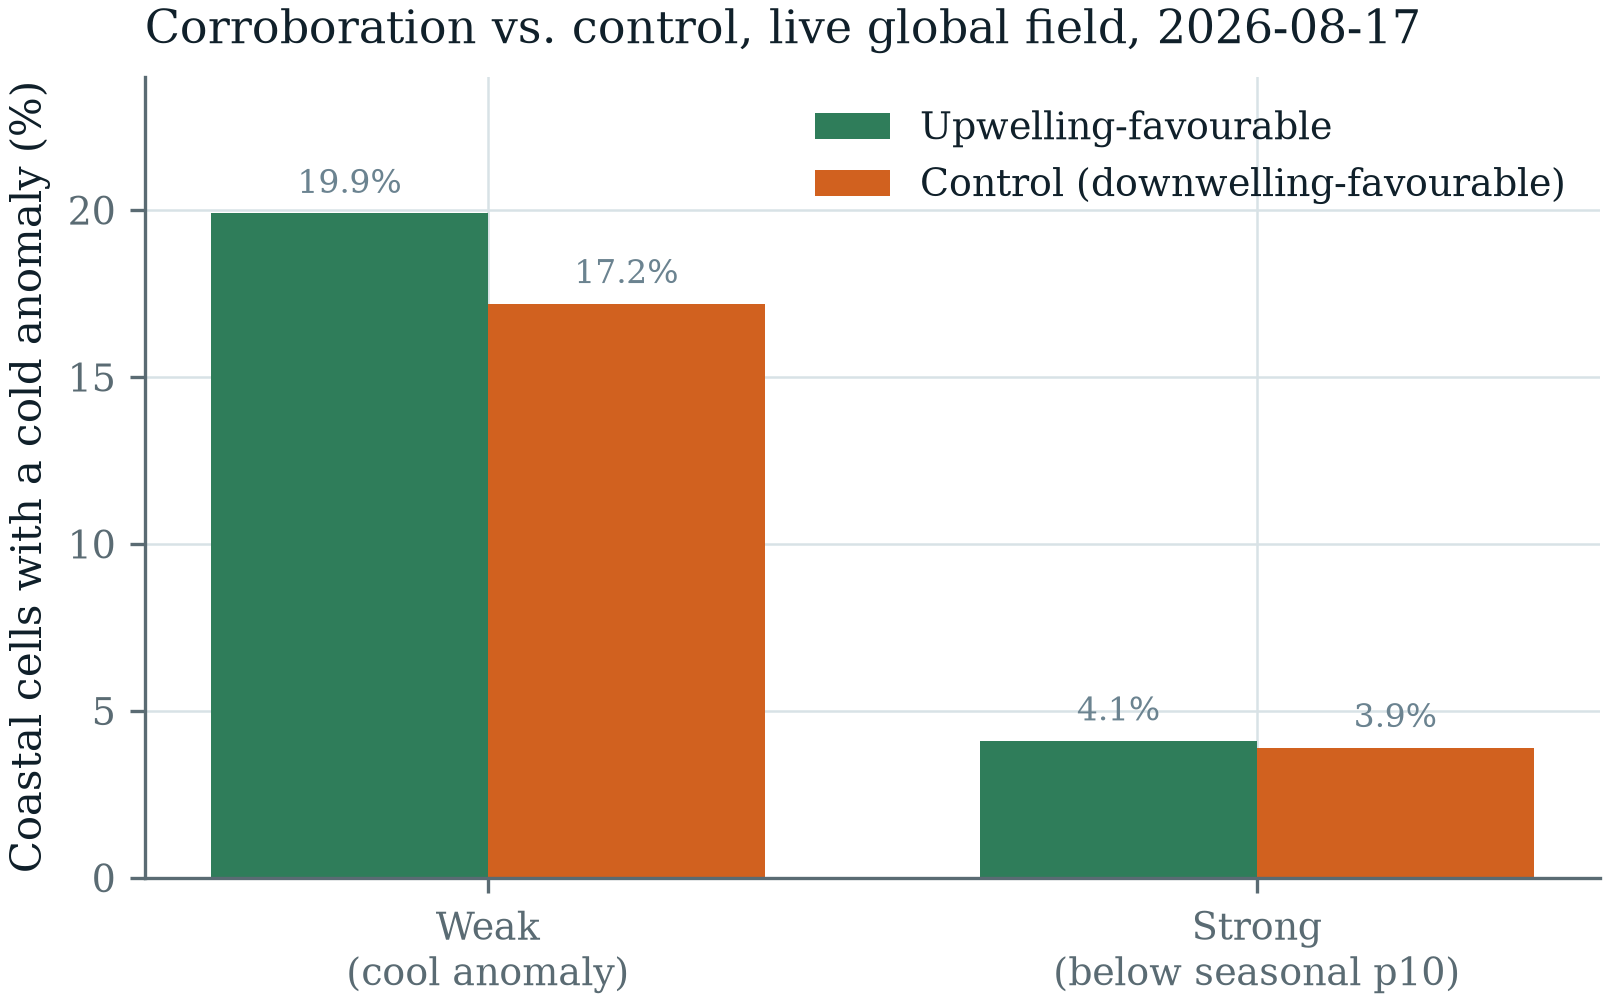
\includegraphics[width=0.85\linewidth]{corroboration_bars}
\caption{The same two tiers as Table~\ref{tab:headline}, plotted: favourable
coasts (green) against the downwelling-favourable control arm (orange).
Neither tier separates cleanly from its own control.}
\label{fig:headline}
\end{wfigure}

\para{The headline gap is narrow, and narrows further at the stronger test}
Table~\ref{tab:headline} reports the live global measurement. At the weak,
mean-based tier, \UpwellFavourWeak{}\% of upwelling-favourable coastal cells
carried a cold anomaly for the season, against \UpwellControlWeak{}\% of
downwelling-favourable cells --- a gap of \UpwellGapWeak{} percentage points.
At the strong, percentile-based tier the gap narrows to \UpwellGapStrong{}
points (\UpwellFavourStrong{}\% against \UpwellControlStrong{}\%). The mean
SST anomaly itself is \emph{positive} on both arms that day --- $+\UpwellAnomFavour{}\si{\celsius}$
under favourable wind, $+\UpwellAnomControl{}\si{\celsius}$ under downwelling
--- so the coastal band as a whole read warm for the season regardless of
wind regime, and the favourable arm was not even the cooler of the two. No
formal significance test exists anywhere in this codebase for either gap; the
honest statement is that both gaps are small relative to their own
percentages, not that either is statistically indistinguishable from the
other in a sense this measurement was designed to test.

\para{The sign convention is independently regression-tested} Running the
platform's own test suite directly (\texttt{uv run pytest
tests/test\_upwelling.py tests/test\_wind\_history.py -q}) on \AsOf{} passes
all \NTotalUpwellingTests{} tests (\NUpwellingTests{} in
\texttt{test\_upwelling.py}, \NWindHistoryTests{} in
\texttt{test\_wind\_history.py}). The test most directly relevant to this
paper's own construction is a deliberately adversarial fixture: a coastline
placed with land in the \emph{high}-longitude columns and open ocean to the
west, called an eastern boundary --- the geometry of California, Peru,
Namibia, and Somalia --- checked against an equatorward wind that must
upwell there, and mirrored in latitude to confirm the southern hemisphere
reverses sign rather than repeating the northern result. Getting the
coastline's orientation backwards in this fixture is the one error that
would report every upwelling coast on Earth as downwelling while still
producing a field that looks entirely plausible, exactly the failure mode
\S\ref{sec:methods} warns the sign convention is exposed to.

\begin{wtable}
\centering
\tabscale
\caption{The wind-history follow-up, read against the natural day-to-day
spread of the same, unchanged matched configuration (OISST scored against
its own OISST-fitted climatology, instantaneous wind unless noted). Contrasts
are favourable-minus-control fractions, not percentages, and are not
comparable to Table~\ref{tab:headline}'s units. [DATED throughout; the
1.2-day trailing mean row is Artifact-backed infrastructure with a Dated
value.]}
\label{tab:windhistory}
\begin{tabular}{llrr}
\toprule
Date & Wind input & Weak contrast & Strong contrast \\
\midrule
2026-08-17 & instantaneous & \MatchedWeakAugSeventeen{} & \MatchedStrongAugSeventeen{} \\
2026-08-25 & instantaneous & \MatchedWeakAugTwentyFive{} & \MatchedStrongAugTwentyFive{} \\
2026-08-28 & instantaneous & \WindHistoryWeakInstant{} & \WindHistoryStrongInstant{} \\
2026-08-28 & \WindHistoryActualWindowDays{}-day trailing mean & \WindHistoryWeakTrailing{} & \WindHistoryStrongTrailing{} \\
\bottomrule
\end{tabular}
\end{wtable}

\begin{wfigure}
\centering
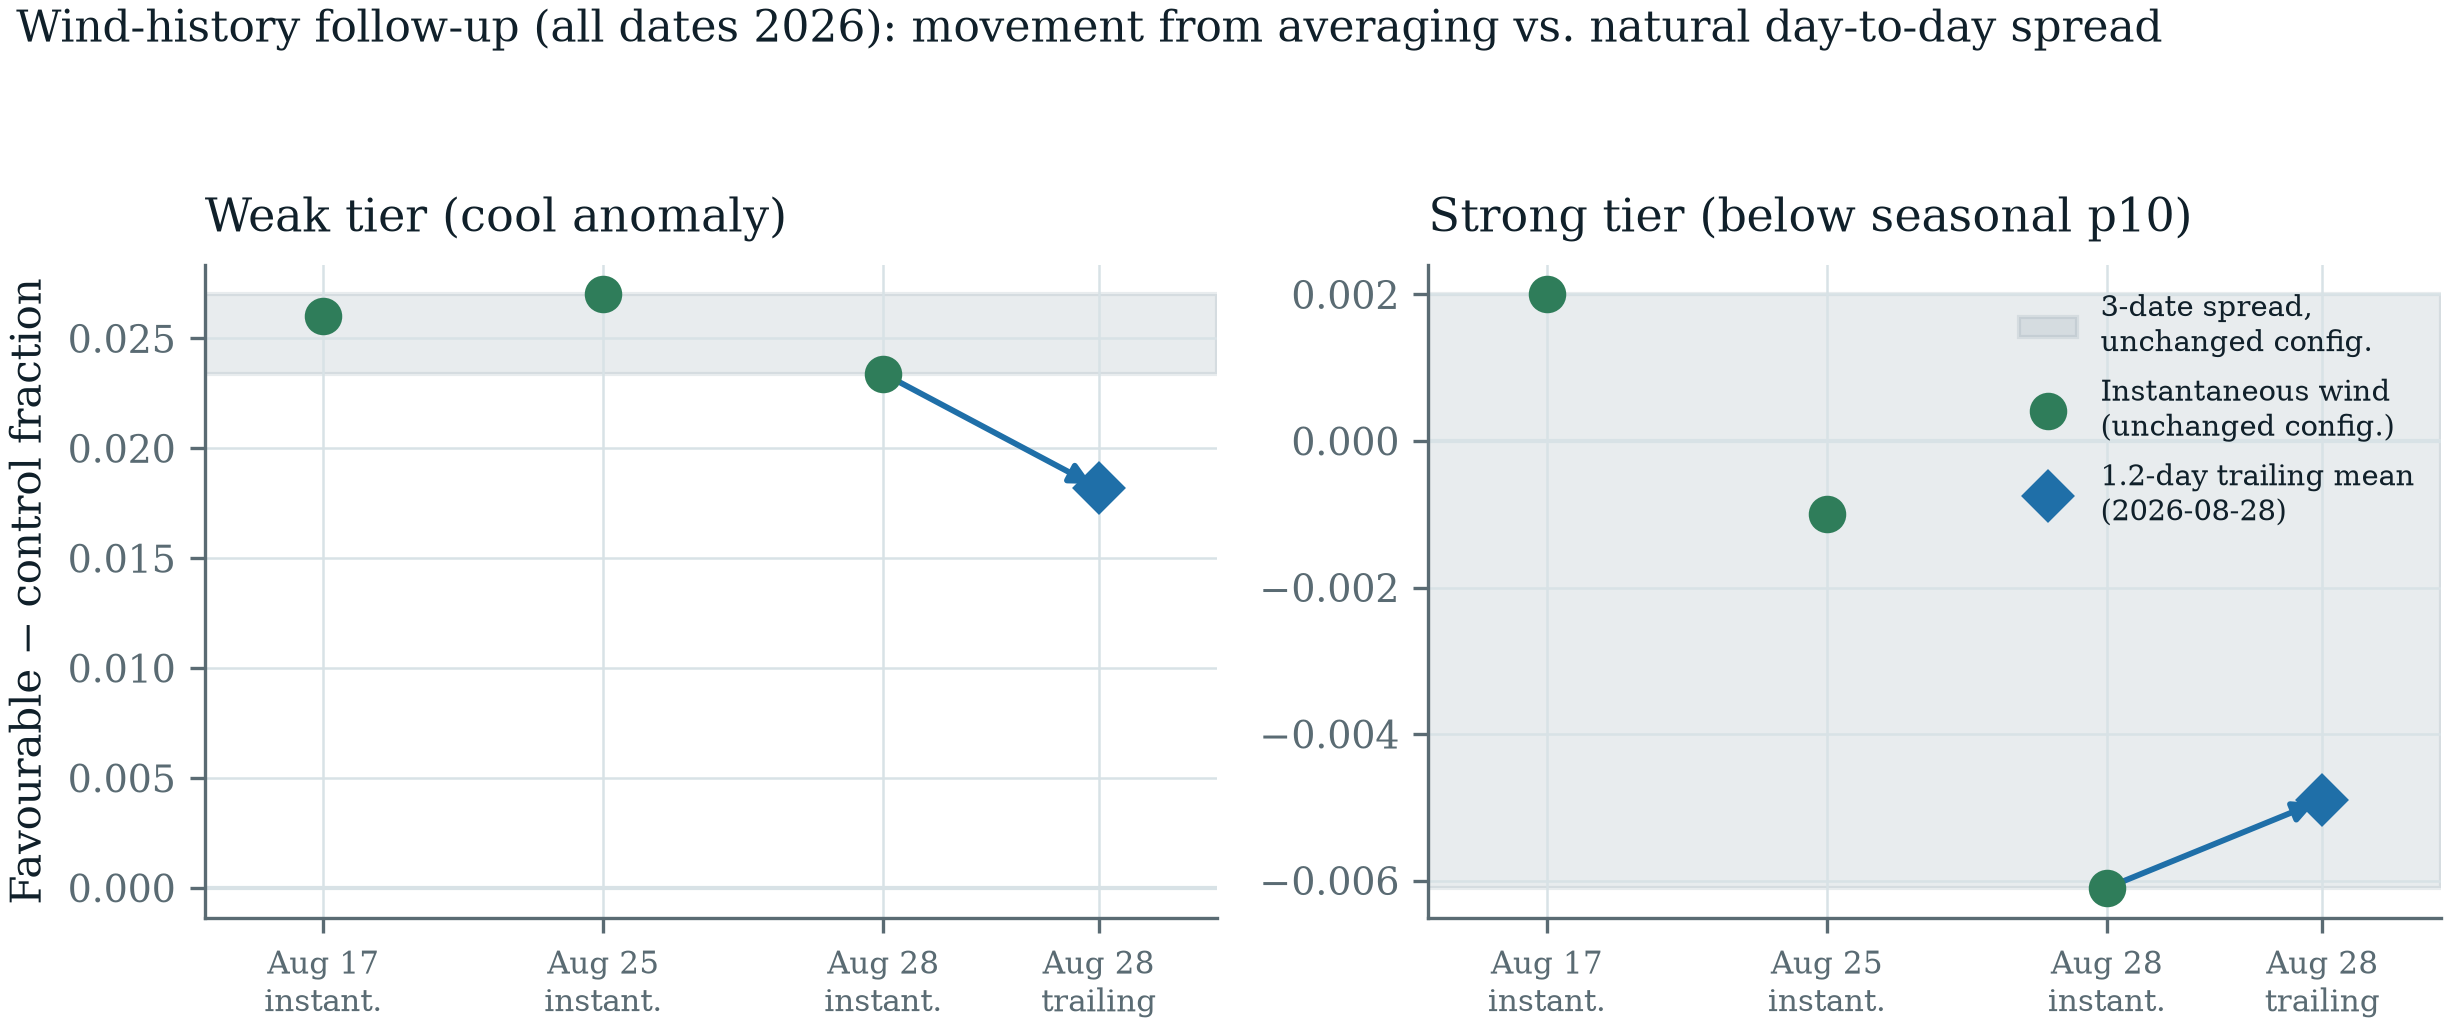
\includegraphics[width=0.85\linewidth]{wind_history_spread}
\caption{Each panel plots one tier's contrast across four measurements: three
dates of the identical, unchanged matched configuration (circles) and the
2026-08-28 trailing-mean arm (diamond), connected to its own day's
instantaneous value (arrow). The shaded band spans the three-date range of
the unchanged configuration -- the natural day-to-day spread the
wind-averaging movement has to be read against.}
\label{fig:windhistory}
\end{wfigure}

\para{The wind-history follow-up does not widen the gap} Research notes
associated with this detector, written before this paper's own verification
pass, name a rolling wind history as the natural next experiment and
describe it as not yet built. It has since been built
(\S\ref{sec:methods}) and measured, on 2026-08-28, against a real backfilled
\WindHistoryActualWindowDays{}-day window. Table~\ref{tab:windhistory}
reports the result beside two earlier measurements of the identical matched
configuration, with nothing about the method changed between them, so the
table also shows how much this configuration moves on its own from one live
snapshot to the next. On the weak tier, the trailing mean moves the contrast
from \WindHistoryWeakInstant{} to \WindHistoryWeakTrailing{}, a movement of
\WindHistoryWeakMovement{} --- toward zero, not away from it, and somewhat
larger than the \WeakCrossDateSpread{} spread the same unchanged
configuration already shows across the two earlier dates in the table. On
the strong tier the trailing mean moves the contrast from
\WindHistoryStrongInstant{} to \WindHistoryStrongTrailing{}, a movement of
only \WindHistoryStrongMovement{} --- smaller than the
\StrongCrossDateSpread{} spread the unchanged configuration already shows
across its own three measurement dates, which itself \emph{changes sign}
(\MatchedStrongAugSeventeen{}, \MatchedStrongAugTwentyFive{},
\WindHistoryStrongInstant{}) with nothing about the method varied at all.
Averaging the wind over the available window neither widens the gap this
paper's control arm shows to be narrow, nor moves by more than the
day-to-day noise the same test already exhibits when nothing is changed.

\section{Discussion}
\label{sec:discussion}

\para{A corroboration rate needs its control before it means anything}
\UpwellFavourWeak{}\% read alone is a confident-sounding number: a fifth of
every upwelling-favourable coast was cool for the season. Scored beside
\UpwellControlWeak{}\% on coasts where a cold anomaly is not expected, the
same number shows an agreement barely wider than what the same test finds
where it should find nothing. This is the paper's central point stated as
plainly as the measurement supports: the wind index and the SST observation
are two real, independently computed claims about the same coast, and their
coincidence on 2026-08-17 is weak evidence connecting them, not because
either measurement is wrong, but because a single day's snapshot at this
resolution and this SST lag does not carry much evidential weight either
way.

\para{What the wind-history follow-up actually shows} It would overstate
this paper's own evidence to read Table~\ref{tab:windhistory} as proof that
no wind-averaging window would help; it is one measurement at one window
length, \WindHistoryActualWindowDays{} days against an originally targeted
\WindHistoryTargetWindowDays{}, obtained because that is what a real
backfill of the platform's own wind cache produced. What it does show,
honestly stated, is that this specific attempt did not widen the gap, and
that the size of its effect is not clearly distinguishable from the
day-to-day variation the identical, unmodified configuration already
displays when measured on different dates with nothing about the method
changed. The strong tier's own cross-date instability --- positive on
2026-08-17, negative on 2026-08-25, more negative still on 2026-08-28, with
no change to the method between any of those three measurements --- is
itself informative: it shows the strong tier is dominated by noise at the
scale these measurements operate at, which is exactly the condition under
which asking that tier to demonstrate a wind-averaging effect is unlikely to
succeed regardless of whether integrating the wind over days is physically
the right idea. Table~\ref{tab:windhistory}'s honest reading is "tried once,
real data, did not help" --- not "proven not to help at any window length."

\para{One run, read for two different questions} The 2026-08-28 measurement
in Table~\ref{tab:windhistory}'s last two rows is the identical run a
contemporaneous companion draft in this research program analyses as its own
control measurement, for a different purpose: that draft holds the SST
product and its climatology fixed throughout and uses this same
instantaneous-versus-trailing-mean comparison to rule out instantaneous wind
sampling as an alternative explanation for a cross-SST-product mismatch it
measures separately. Both readings are compatible and draw on the same four
numbers; neither supersedes the other, since the questions are different ---
whether wind averaging explains an unrelated cross-product inversion, versus
whether wind averaging rescues this paper's own control-arm gap. Reporting
both without saying they share a measurement would understate how much
independent evidential weight one dated run of a live pipeline actually
carries.

\para{The regression test protects the sign, not the corroboration strength}
\NTotalUpwellingTests{} passing tests, including the adversarial
eastern-boundary/hemisphere fixture described in \S\ref{sec:results},
establish that the index's own sign convention is correct and will stay
correct under refactoring. That is a different, narrower guarantee than "the
corroboration is strong," and this paper is explicit that the two should not
be conflated: a detector can have a perfectly reliable sign convention and
still show a control-arm gap too narrow to support a causal claim on a given
day, because the sign convention and the corroboration strength are answers
to different questions. The platform's response to the second, weaker
finding is not to remove the corroboration --- a real, if weak, coincidence
is still worth reporting --- but to compute and return \texttt{control\_cool\_fraction}
with every response, so a caller reading the corroborated fraction is never
more than one field away from the number that says how much of it might be
chance.

\section{Limitations}
\label{sec:limitations}

Both of this paper's central measurements are single, dated, live
observations of moving fields, not repeated-sampling or formally tested
results: no significance test exists anywhere in this codebase for the
2026-08-17 headline gap, the three-date spread in
Table~\ref{tab:windhistory}, or the wind-history movement, and this paper
reports raw gaps and spreads rather than a p-value or confidence interval it
cannot honestly produce. The wind-history follow-up specifically reached
only a \WindHistoryActualWindowDays{}-day window against the
\WindHistoryTargetWindowDays{}-day window originally targeted, limited by a
real, documented gap in the underlying wind cache rather than by a design
choice; a longer window, or repeated sampling across several separate days
and seasons for either the headline measurement or the follow-up, remains
untried. The infrastructure to run either --- \texttt{services/wind\_history.py},
\texttt{upwelling.detect\_from\_history}, and the backfill script --- is
already built and tested, which makes either extension a re-run rather than
a re-build, but neither has been done as of \AsOf{}. Only the weak tier's
control fraction is a field the live API exposes; a caller relying on the
shipped response alone sees the weak-tier comparison this paper reports but
not the strong-tier or mean-anomaly evidence, both of which currently exist
only as dated numbers in the detector's own source comments. The third,
chlorophyll-based corroborating leg the platform's own documentation
describes as a long-standing goal remains blocked on the same missing input
it always was: there is no resident chlorophyll field and no long-record
chlorophyll baseline to fit a climatology on, so a three-way corroboration
(wind, SST, and biological response) is not yet possible to build, let alone
measure. Finally, this is one detector, one SST product, one climatology,
and one geographic scope (the global coastal band at $\sim$0.25-degree
resolution); whether a control-arm gap this narrow is characteristic of
wind-driven upwelling corroboration generally, or specific to this
platform's product choices and measurement dates, is not established by a
single running system.

\section{Conclusion}

A wind-derived upwelling index corroborated against an independent cold-SST
observation reads, on its own, as confirmation: \UpwellFavourWeak{}\% of
favourable coastal cells were anomalously cool for the season on the day
measured. Scored identically on a control arm where that signal is not
expected --- downwelling-favourable coasts --- the same test returns
\UpwellControlWeak{}\%, a gap of \UpwellGapWeak{} points that narrows to
\UpwellGapStrong{} at the stronger, percentile-based tier, with the mean SST
anomaly warmer than the seasonal average on both arms that day. A follow-up
experiment this platform's own prior account named as the natural next step
--- integrating the wind input over a real, multi-day trailing window rather
than scoring one instantaneous snapshot --- has since been built and
measured, and does not widen the gap; its movement is not clearly
distinguishable from the day-to-day variation the identical, unmodified
configuration already shows across separate measurement dates. Detector
corroboration is usually reported as a single agreement rate and left there.
The discipline this paper applies, twice, is cheap, computed from data
already in hand, and available to any detector that corroborates one signal
against a second: score the same test where the effect is not expected, and
read the gap, not the level.


\section*{Reproducibility}
The detector is \texttt{backend/services/upwelling.py}; the corroboration
test and its control arm are \texttt{UpwellingField.corroboration()},
consumed by \texttt{GET /api/ocean/upwelling\{,/point,/cells\}}. The
2026-08-17 headline measurement and the 2026-08-17/2026-08-25 matched-configuration
values in Table~\ref{tab:windhistory} are recorded directly in that module's
and in \texttt{backend/services/sst\_anomaly.py}'s own module docstrings; both
are reproducible on demand by running \texttt{scripts/measure\_sst\_corroboration.py}
against a live Copernicus/OISST snapshot, but no output file is committed for
either date. The hemisphere/eastern-boundary regression suite is
\texttt{backend/tests/test\_upwelling.py} (\NUpwellingTests{} tests) and
\texttt{backend/tests/test\_wind\_history.py} (\NWindHistoryTests{} tests),
all \NTotalUpwellingTests{} passing as of \AsOf{} via \texttt{uv run pytest
tests/test\_upwelling.py tests/test\_wind\_history.py -q}. The wind-history
follow-up is \texttt{backend/services/wind\_history.py} and
\texttt{upwelling.detect\_from\_history}, backfilled by
\texttt{scripts/backfill\_wind\_history.py} and measured by
\texttt{scripts/measure\_wind\_history\_corroboration.py}; its 2026-08-28
numbers are recorded in \texttt{sst\_anomaly.py}'s docstring and in
\texttt{DONE.md}'s ``A rolling wind history'' entry, with no stored output
file committed. Every number in this paper was re-verified against those
sources, and every relevant test was re-run, as of \AsOf{}.

\bibliographystyle{splncs04}
\bibliography{../shared/references}

\end{document}
